\subsection{Bidirectional transformation with TGGs}

\subsubsection{Possibilities with TGGs and Moflon}
\label{TGG_overview_chapter}
For bidirectional transformations Tripple Graph Grammars (TGGs) are used. This three graph based transformation contains a source, target and correspondency graph, from which the transformation is derived. For more information about this transformation we refer you to work through Part IV of our handbook.
\newline
With this transformation there are many possible applications. In Fig.~\ref{Tgg_overview} is an overfiew of some possibilities, which are treated in the handbook.

\begin{figure}[htbp]
	\centering
  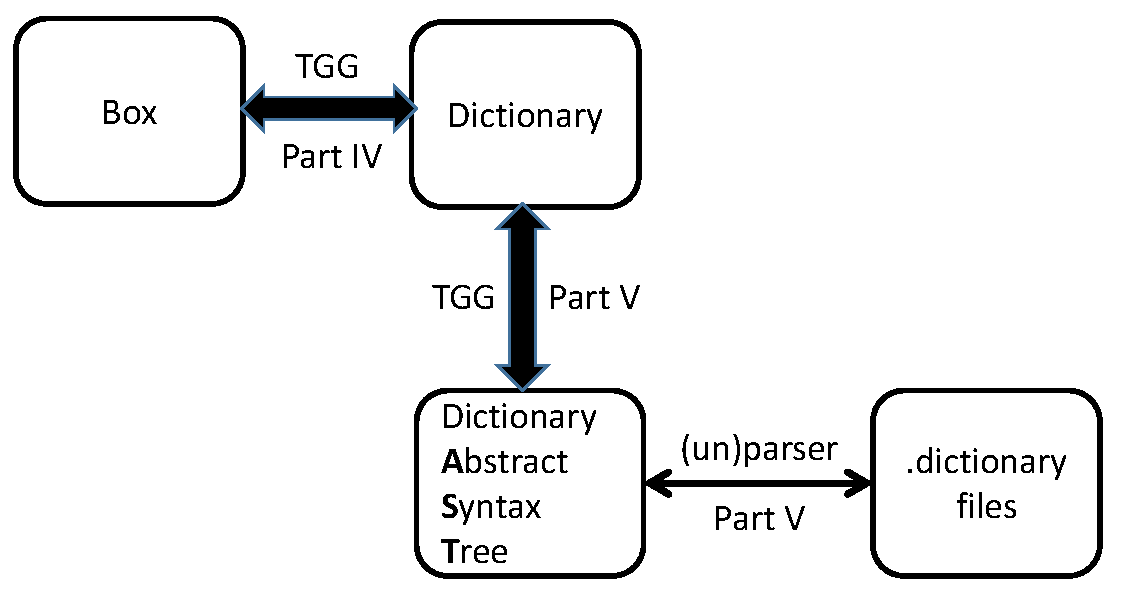
\includegraphics[width=0.8\textwidth]{TGG_overview.pdf}
	\caption{Overview of TGG usage} 
	\label{Tgg_overview} 
\end{figure}


You are able to create bidirectional transformations between different metamodels, which is handled in Part IV, or even transform between an Abstract Syntax Tree (AST) and a metamodel. Additional you can also use an (un)parser to transform it into textfiles and wice versa. The latter is examined in Part V.

%---------------------------------------------------------------------------------------------------

\subsubsection{Implementation of a TGG rule}
Now, after you have a brief overfew of TGGs, we will have a look at how you can use this in Moflon for creating bidirectional transformations. For this we will examine one TGG rule as an example.

\begin{itemize}

\item Open the \texttt{CardToEntryRule} in \texttt{Learning\-Box\-To\-Dictionary\-Integra\-tion/\-Rules} (Fig.~\ref{ea:openTGG_rule}).

\begin{figure}[htbp]
	\centering
  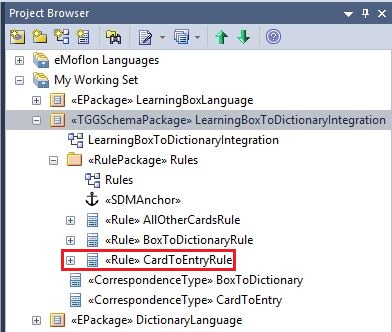
\includegraphics[width=0.6\textwidth]{ea_select_tgg_rule}
	\caption{Open the \texttt{CardToEntryRule}} 
	\label{ea:openTGG_rule} 
\end{figure}

\end{itemize}

In Fig.~\ref{ea:TGG_rule} you see the \texttt{Card\-To\-Entry\-Rule}. In this rule we describe the transformation between card and entry. Like as at the SDM before, black elements are here also context elements. In this case we have \texttt{box}, its correspondency \texttt{dictionary} and \texttt{partition0} as context elements. Green elements are the elements, which are transformed in this rule, thus \texttt{card} and \texttt{entry}.
\newline
As mentioned before, TGG is a three graph based language. One source and target graph, which are left and right in Fig.~\ref{ea:TGG_rule}, and a correspondency graph in the middle. For the transformation between \texttt{card} and \texttt{entry} we have the correspondency \texttt{cardToEntry}.
\newline
To set the attribute values we solving a \texttt{constraint satisfaction problem} (CSP). This is the black box at the bottom of the diagram. Here you have different possibilities to set or create the values. To know what you can do exactly and more details to the transformation with TGGs, we refer you to work through Part IV and V of our handbook.

\begin{figure}[htbp]
	\centering
  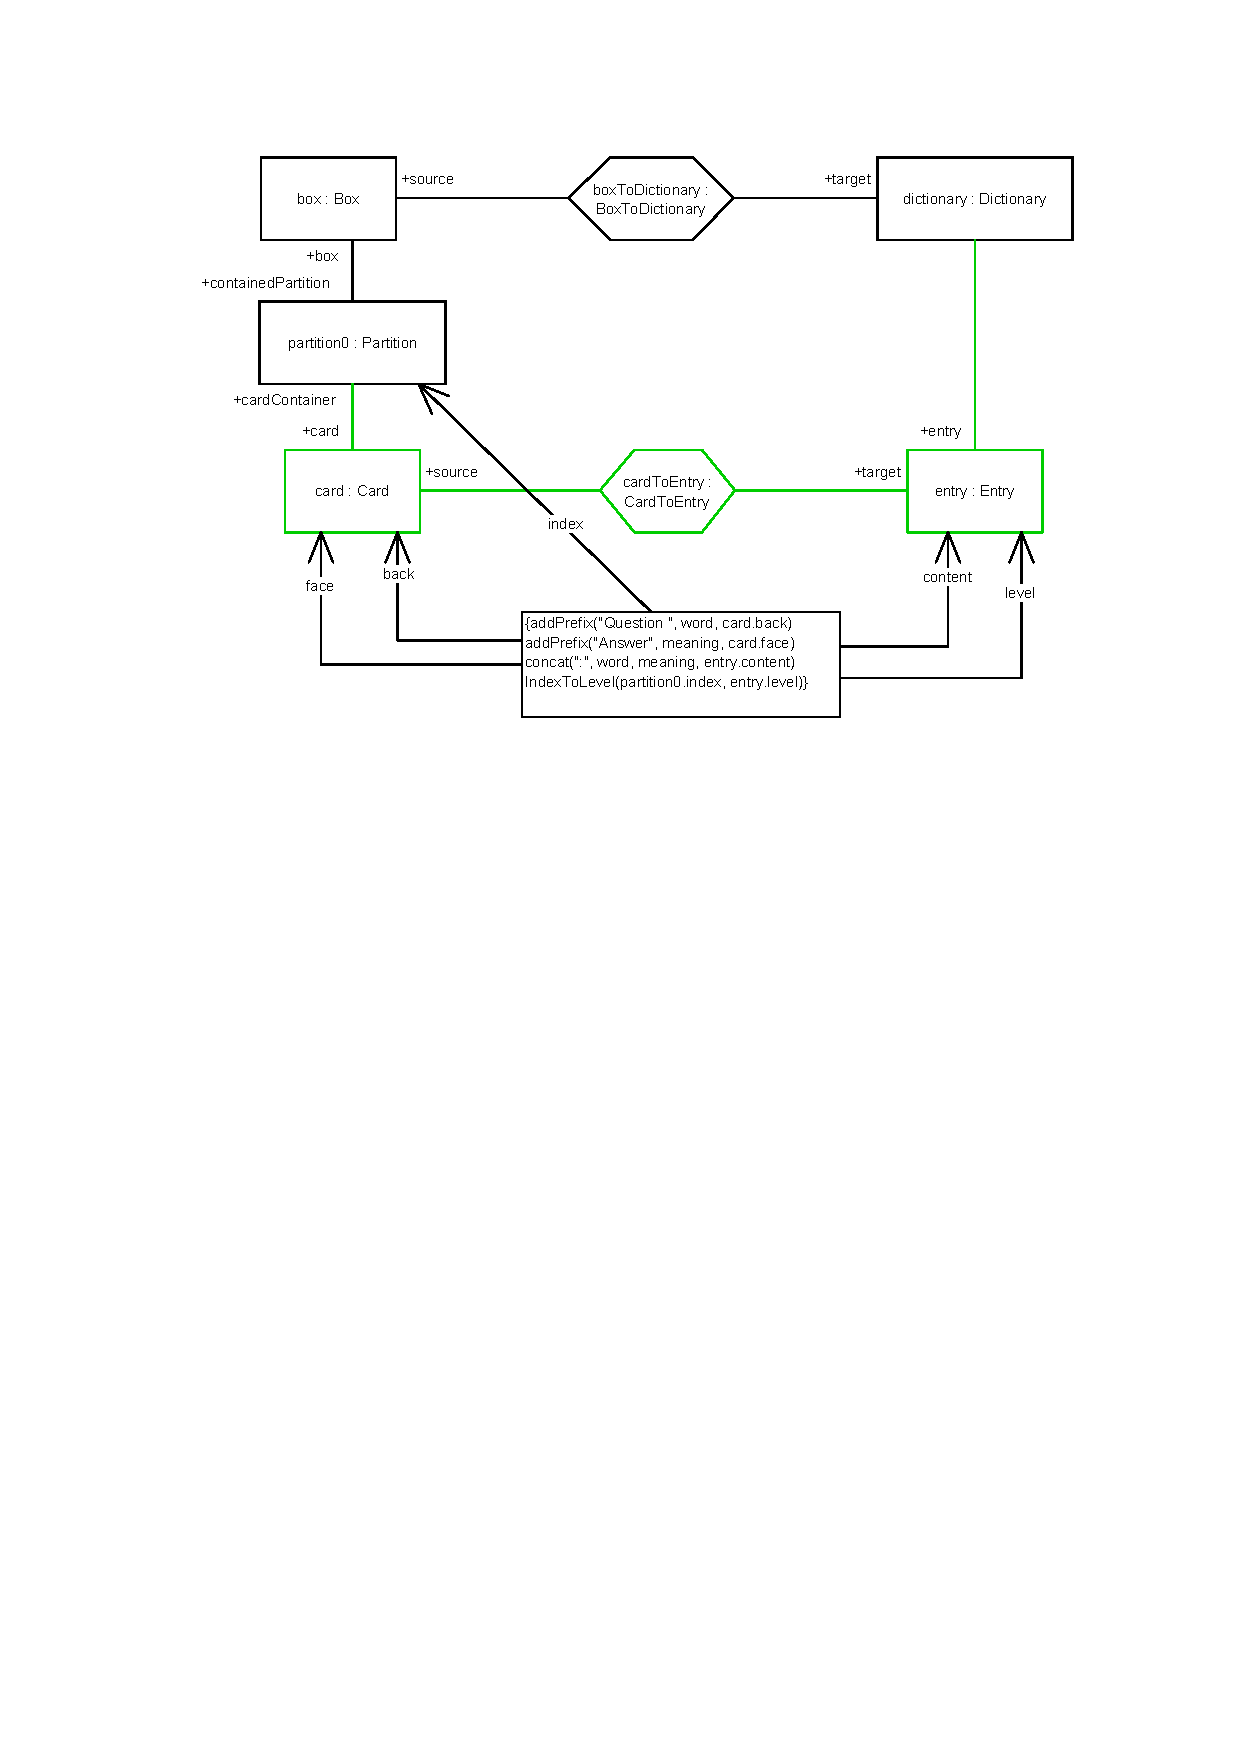
\includegraphics[width=1\textwidth]{TGG_rule}
	\caption{TGG rule \texttt{CardToEntryRule}} 
	\label{ea:TGG_rule} 
\end{figure}